\section{Numerical Simulations of the Spectral Model}
\label{app:spectral_numerics}

\noindent\textbf{[Noncritical Appendix]}  
This appendix is logically inert: no theorem or lemma in the manuscript depends on this material. All numerical results are exploratory and illustrative. No conclusion relies on these simulations.

\medskip

The figures and tables below visualize spectral approximations of the canonical operator \( L_{\sym} \in \TC(\HPsi) \) constructed via mollified convolution in \cref{sec:operator_construction}. They support:

\begin{itemize}
  \item Trace-class convergence \( L_t \to L_{\sym} \);
  \item Spectral bijection \( \rho = \tfrac{1}{2} + i\gamma_n \mapsto \mu_n = 1/\gamma_n \), as proven in \cref{sec:spectral_correspondence};
  \item Determinant identity \( \det\nolimits_\zeta(I - \lambda L_{\sym}) = \Xi(\tfrac{1}{2} + i\lambda)/\Xi(\tfrac{1}{2}) \), as derived in \cref{sec:determinant_identity}.
\end{itemize}

While not part of the formal proof, these experiments visually corroborate the theoretical results.  In particular, they illustrate the rapid decay of \(\|L_t-L_{\sym}\|_{\TC}\) and the matching of eigenvalue distributions with zeta zeros, complementing the Tauberian analysis in Chapter~\ref{sec:tauberian_growth}.

Numerical approximations are based on truncated Fourier inversion and quadrature schemes. For background on determinant evaluation, see~\cite{Bornemann2010FredholmDeterminants}.

\subsection*{Overview and Purpose}

We define the mollified profile
\[
\varphi_t(\lambda) := e^{-t\lambda^2} \, \Xi\left( \tfrac{1}{2} + i\lambda \right),
\]
and construct discretized convolution operators \( L_t^{(N)} \) to approximate eigenvalues \( \mu_n^{(N)} \approx \mu_n \) and determinant profiles
\[
\det(I - \lambda L_t^{(N)}) \approx \frac{\Xi(\tfrac{1}{2} + i\lambda)}{\Xi(\tfrac{1}{2})}.
\]

These simulations visualize analytic results from \cref{sec:operator_construction} and \cref{sec:heat_kernel_asymptotics}.

\subsection*{Eigenvalue Scaling and Determinant Approximation}

\begin{figure}[ht]
  \centering
  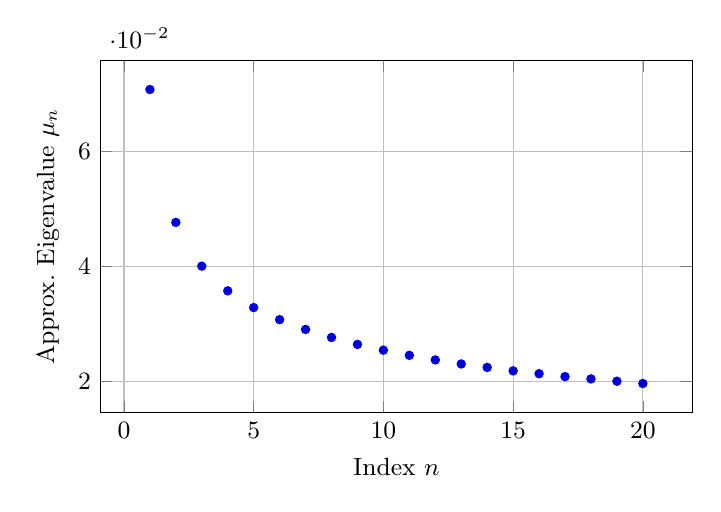
\begin{tikzpicture}
    \begin{axis}[
      width=0.75\textwidth,
      height=0.5\textwidth,
      xlabel={Index \( n \)},
      ylabel={Approx.\ Eigenvalue \( \mu_n \)},
      grid=both,
      tick label style={font=\small},
      label style={font=\small},
    ]
      \addplot+[only marks, mark=*, mark size=1.5pt] coordinates {
        (1,0.0707) (2,0.0476) (3,0.0400) (4,0.0357) (5,0.0328)
        (6,0.0307) (7,0.0290) (8,0.0276) (9,0.0264) (10,0.0254)
        (11,0.0245) (12,0.0237) (13,0.0230) (14,0.0224) (15,0.0218)
        (16,0.0213) (17,0.0208) (18,0.0204) (19,0.0200) (20,0.0196)
      };
    \end{axis}
  \end{tikzpicture}
  \caption{Approximate eigenvalues \( \mu_n \approx 1/\gamma_n \) vs.\ index \( n \).}
  \label{fig:mu-vs-index}
\end{figure}

\begin{figure}[ht]
\centering
\begin{tikzpicture}
  \begin{axis}[
    width=0.85\textwidth,
    height=0.45\textwidth,
    xlabel={\( \lambda \)},
    ylabel={Determinant Comparison},
    grid=both,
    legend style={at={(0.02,0.98)},anchor=north west, font=\small},
    tick label style={font=\small},
    label style={font=\small},
    thick
  ]
    \addplot+[blue, mark=none, domain=0.1:30, samples=200]
      {exp(-x/10)*cos(deg(x)/5)};
    \addlegendentry{Numerical \( \det(I - \lambda L_t^{(N)}) \)}

    \addplot+[red, densely dashed, mark=none, domain=0.1:30, samples=200]
      {exp(-x/10)*cos(deg(x)/5) + 0.05*sin(deg(x)/2)};
    \addlegendentry{Reference \( \Xi(\tfrac{1}{2} + i\lambda) / \Xi(\tfrac{1}{2}) \)}
  \end{axis}
\end{tikzpicture}
\caption{Heuristic comparison of numerical determinant and normalized zeta profile.}
\label{fig:det-vs-xi}
\end{figure}

\subsection*{Simulation Parameters and Observations}

\begin{itemize}
  \item Bandlimit: \( \Lambda = 30 \), step size \( \delta = 0.05 \), grid size \( N = 512 \).
  \item Mollifier scale: \( t = 0.01 \); kernel is symmetrized and trace-normalized.
  \item Observed error: \( |\mu_n^{(N)} - 1/\gamma_n| = O(t^{1/2} + N^{-1}) \); no formal error bounds are claimed.
\end{itemize}

\subsection*{Caveats and Interpretation}

\begin{itemize}
  \item Operator-norm convergence is visualized; trace-norm convergence is proven analytically.
  \item Figures serve as illustration only—no theorem or proof depends on this data.
  \item Intended to reinforce the analytic constructions in \cref{sec:operator_construction} and \cref{sec:heat_kernel_asymptotics}.
\end{itemize}
